% \Image{Capa do livro (; )}{PNLD2022-021-01.png}

% \Image{Ilustração do livro (; )}{PNLD2022-021-04.png}
% \Image{Ilustração do livro (; )}{PNLD2022-021-05.png}
% \Image{Ilustração do livro (; )}{PNLD2022-021-06.png}


\documentclass[11pt]{extarticle}
\usepackage{manualdoprofessor}
\usepackage{fichatecnica}
\usepackage{lipsum,media9}
\usepackage[justification=raggedright]{caption}
\usepackage[one]{bncc}
\usepackage[lunna]{../edlab}
\usepackage{marginnote}
\usepackage{pdfpages}
\usepackage[printwatermark]{xwatermark}
\newwatermark[pagex=2]{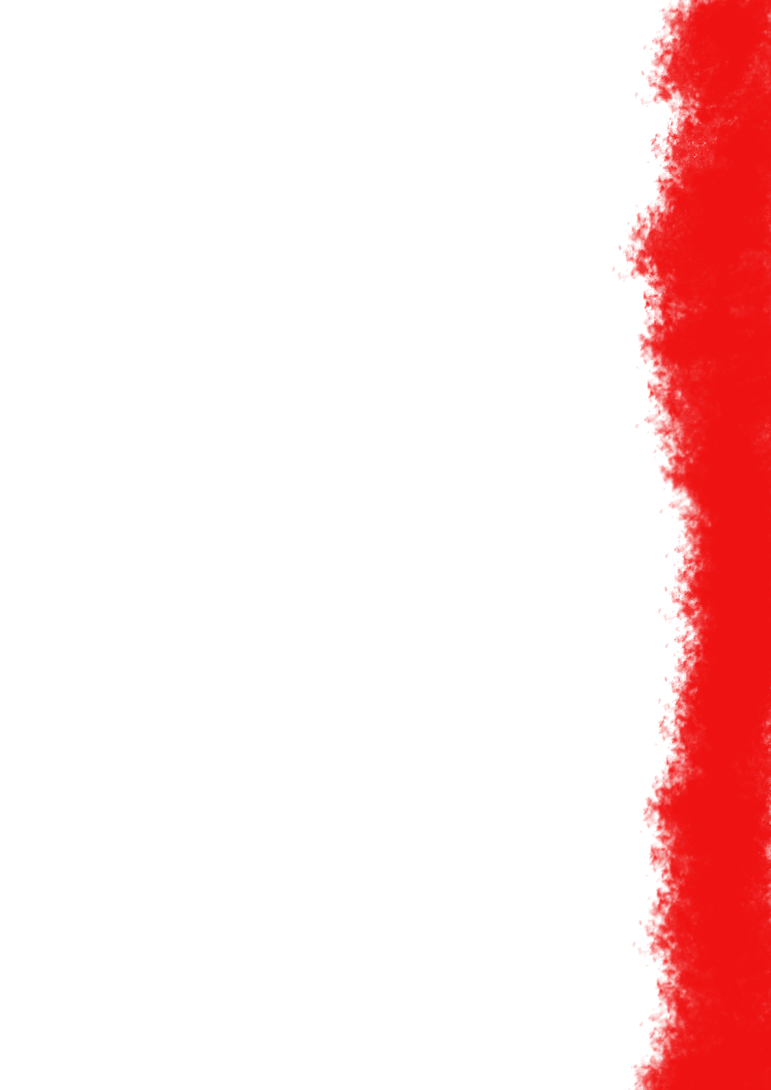
\includegraphics[scale=3.3]{watermarks/test-a.png}}	% página específica
%\newwatermark[oddpages]{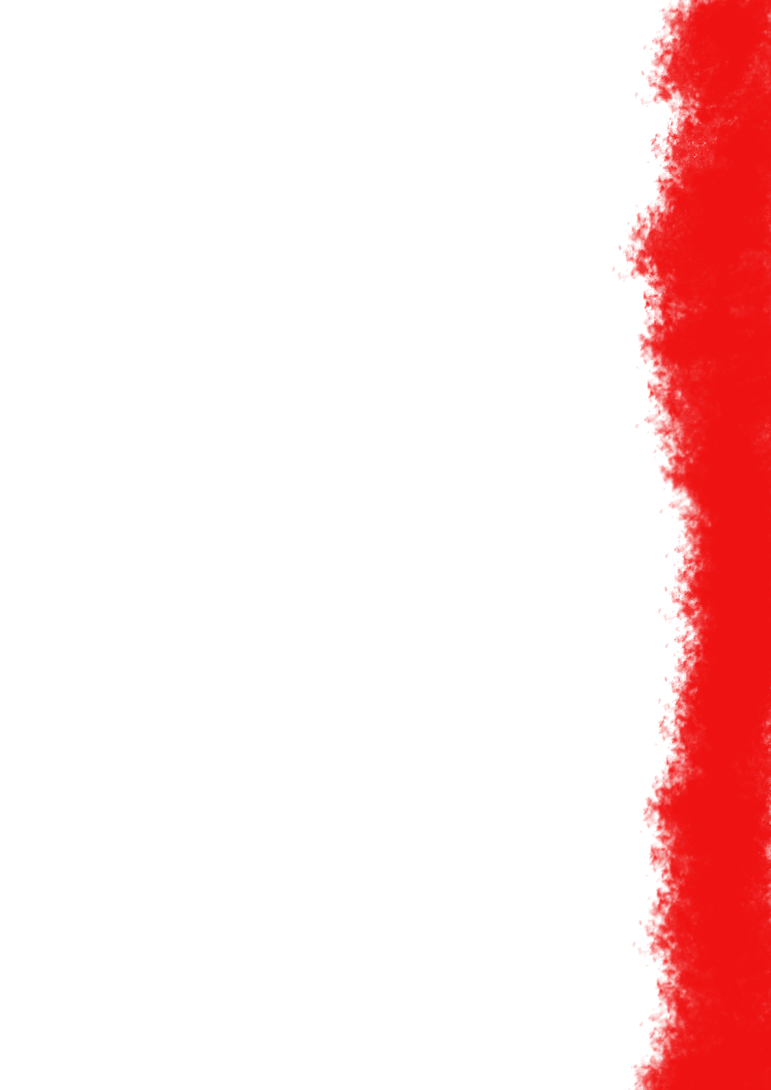
\includegraphics{watermarks/test-a.png}}			% páginas ímpars
%\newwatermark[evenpages]{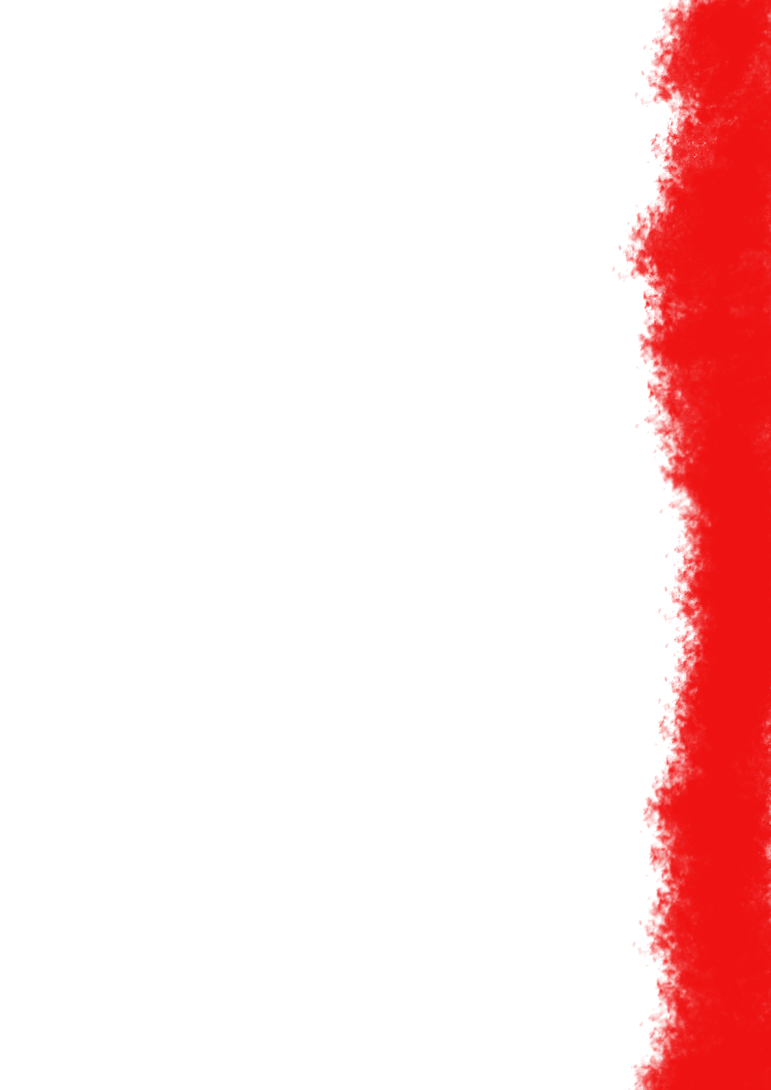
\includegraphics{watermarks/test-a.png}}			% págimas pares
\newwatermark[allpages]{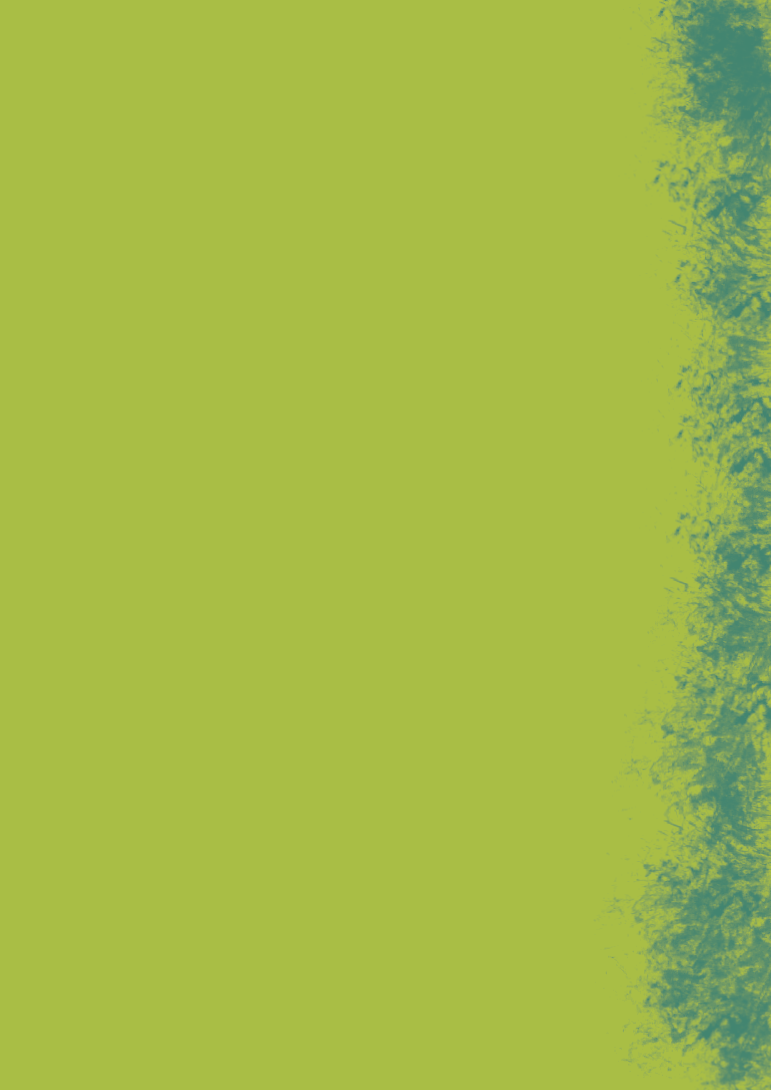
\includegraphics[scale=3.3]{watermarks/test-b.png}}

\pagecolor{cyan!0!magenta!10!yellow!28!black!28!}

\newcommand{\AutorLivro}{Marcelo Cipis}
\newcommand{\TituloLivro}{Palavra-chave}
\newcommand{\Tema}{Quotidiano de crianças nas escolas, nas famílias e nas comunidades}
\newcommand{\Genero}{Poesia}
%\newcommand{\imagemCapa}{./images/PNLD0001-01.png}
\newcommand{\issnppub}{978-65-86497-57-1}
\newcommand{\issnepub}{978-65-86497-73-1}
% \newcommand{\fichacatalografica}{PNLD0001-00.png}
\newcommand{\colaborador}{{Paulo Pompermaier e Renier Silva}}

\begin{document}

\title{\TituloLivro}
\author{\AutorLivro}
\def\authornotes{\colaborador}

\date{}
\maketitle

%\begin{abstract}\addcontentsline{toc}{section}{Carta ao professor}
%\pagebreak

\tableofcontents



\section{Sobre o livro}

%27 caracteres
\paragraph{O livro} 
``Palavra-chave'' é um livro de tom poético que trabalha
com linguagem verbal e não verbal. 
%822 caracteres
\paragraph{Descrição} 
Ao todo são quinze palavras-objetos criadas pelo autor apresentadas
a cada página. As ilustrações misturam elementos das duas partes 
em relação. Por exemplo, o ``carro-girafa'' terá o pescoço longo e 
a cabeça do animal junto à estrutura básica do carro, e assim por diante
com as demais figuras híbridas.

%411 caracteres
\paragraph{Competências} 
Uma das competências mais relevantes trabalhada por este livro
é a que diz respeito à linguagem e à imaginação. 
As crianças em contato com esta obra serão convidadas a experimentar
o aspecto criativo da linguagem que não se limita às regras da
realidade.

A interpretação do código visual 
exige competências que são muito bem desenvolvidas em crianças pequenas: 
observação e imaginação e, portanto, permitem debate e troca de ideias durante 
a leitura. A exploração as ilustrações deste livro com seus alunos, contribuirá 
para o enriquecimento do repertório da criança: desde o vocabulário até o 
olhar artístico que também pode ser afinado ao longo do trabalho.

%862 caracteres
\paragraph{Aprofundamento} Este material tem a 
intenção de contribuir para que você consiga desenvolver um trabalho aprofundado 
com esta obra na sala de aula. Você encontrará informações sobre o autor, sobre 
o gênero e sobre os temas trabalhados ao longo do livro. Apresentaremos também 
algumas propostas de trabalho para a sala de aula que você poderá explorar livremente, 
da forma que considerar mais apropriada para os seus estudantes. Para a prática 
da Literacia Familiar, oferecemos um guia que pode ajudar nas orientações aos 
responsáveis pela criança, para incentivar o gosto pela leitura e contribuir para 
que os estudantes desenvolvam em casa habilidades que serão importantes no momento 
da alfabetização. Por fim, você encontrará sugestões de livros, artigos e sites 
selecionados para enriquecer a sua experiência de leitura e, 
consequentemente, a de seus estudantes.



\section{Sobre o autor}

\Image{Foto do autor e ilustrador (Arquivo pessoal)}{PNLD2022-021-02.png}

%532 caracteres
\paragraph{O autor} 
Marcelo Cipis nasceu em São Paulo, em 1959. 
Ingressou no mundo das artes plásticas em 1968, com participação em ateliês 
livres e aulas com artistas de diferentes modalidades. Atua sobretudo como 
ilustrador, desenhista e pintor deste 1977, tendo realizado trabalhos para 
livros, revistas e jornais.
%313 caracteres
\paragraph{Publicações} 
Além de ter trabalhado na capa e ilustrações de diversos livros, 
publicou \emph{Era uma vez um livro}, pela Companhia das Letrinhas, \emph{530g de ilustrações}, pelo Ateliê Editorial e, com Antônio Malta, \emph{Viver é... e Namorar é...}, pela Martins Fontes.
%358 caracteres
\paragraph{Currículo} 
Formado em arquitetura pela fau-usp em 1982, participou dos Salões de Arte 
Contemporânea de São Paulo nos anos 1980 e da 21ª Bienal de São Paulo em 1991, 
além de outras mostras e workshops no Brasil e no exterior. Recebeu o Prêmio 
Jabuti de Ilustração em 1994 e uma bolsa da Pollock-Krasner Foundation em 2000, 
entre outros. Suas obras exploram diferentes combinações de formas geométricas 
e cores na representação lúdica de corpos e espaços.

\section{Sobre o gênero}

%55 caracteres
\paragraph{O gênero} O gênero deste livro é \textit{poesia}. 

\Image{O gênero poético incentiva a curiosidade e a imaginação. (LACMA/Remedios Varo; CC BY-NC 2.0)}{PNLD2022-021-07.png}

%596 caracteres
\paragraph{Descrição} A poesia é um gênero que se apresenta não de forma
linear, mas espiral. Talvez por isso as crianças se identifiquem
tanto com este gênero. Além disso, ela possibilita o trabalho com
o lúdico por meio do jogo com palavras e sons. A língua deixa de
ser um mero instrumento para a comunicação e passa a ser percebida
como fonte de prazer estético. Está no campo da poesia a formação da personalidade
humana, aquilo que foge às normas moralizantes e os conteúdos mais
práticos e ``úteis'' para nossa sociedade. 

%603 caracteres
\paragraph{Interação} A leitura e escuta de frases poéticas 
formuladas por uma criança de três anos, como é o caso de ``Frases de Tomé aos três anos'',
convida crianças e adultos para entrar neste jogo de criação de novos sentidos
para as coisas. É neste ambiente de liberdade criativa que crianças e adultos devem
interajir, sem que haja coerção da imaginação de nenhuma das partes. 


%862 caracteres
\paragraph{Competências} No trabalho com este livro, as crianças são 
estimuladas a explorar olhares, gestos, expressões, sons da língua, 
rimas, imagens, textos escritos e ilustrações além dos sentidos das palavras, 
apropriando-se desses elementos para criar novas falas, narrativas, relações 
e imagens sem se preocupar com as regras estabelecidas na linguagem.



\section{Temas}


\subsection{Quotidiano de crianças nas escolas; nas famílias e nas comunidades (urbanas e rurais)}

%136 caracteres
\paragraph{Abordagem} 
Apresentação de palavras e objetos do quotidiano.
%206 caracteres
\paragraph{Descrição} 
A cada página, uma palavra e um objeto do quotidiano das crianças são apresentados
de forma incomum: fundidos. A ilustração que sempre acompanha os temos unidos
por um 
%275 caracteres
\paragraph{Competências} Este tema relaciona-se, principalmente,
ao campo da experiência ``Escuta, fala, pensamento e imaginação''
descrito pela \textsc{bncc}, que explora a experiência da criança 
com a linguagem verbal em diálogo com outras linguagens, 
desde o nascimento, de modo a ampliar não apenas essa linguagem, 
mas também o pensamento e a imaginação.

\section{Modelagem de aula}
A seguir você encontrará a descrição de uma aula modelo como exemplo 
prático de exploração do livro com estudantes. Esta seção apresentará 
orientações sobre como organizar a sala de aula para receber os 
estudantes, exercitar a interação verbal e prepará-los para o 
momento da leitura.

Em seguida, você encontrará a \textbf{Leitura dialogada}, um 
tópico destinado a te orientar para o momento específico da 
leitura com os estudantes. Por fim, no tópico 
\textbf{Propostas de atividades}, você encontrará ideias 
de práticas que pode explorar com as crianças em sala de 
aula após a leitura. 

Essas atividades podem ser trabalhadas de acordo com a 
disponibilidade do seu cronograma e fique à vontade para adaptá-las 
da forma que achar melhor para os seus estudantes. Cada turma é única 
e o seu conhecimento prático das características de cada aluno será 
essencial para definir a melhor forma de aplicar essas ideias. 

O objetivo deste manual é oferecer algumas ideias 
e inspirações para um trabalho que pode ser desenvolvido tanto 
a curto, quanto a médio e longo prazo. Sinta-se a vontade para 
personalizar a aula e torna-la sua, aplicando seus conhecimentos, sua 
personalidade e aproveite para fortalecer 
seu vínculo com a turma.


\subsection{Antes de ler}

\BNCC{EI03ET01}
\BNCC{EI03ET05} 
\BNCC{EI03EF02} 
\BNCC{EI03EF07}

%Alterar o nível escolar nesse parágrafo.
Como este trabalho será realizado com crianças da \textbf{Pré-escola}, 
que ainda não têm muita intimidade com o livro enquanto objeto, você terá o 
papel de mediar este contato. 

Nosso objetivo é que os próprios estudantes possam manusear 
e explorar o livro de forma autônoma, mas, para que isto aconteça, você 
pode ajudar a tornar o caminho mais convidativo com atividades que tenham 
intencionalidade educativa. 

A \textsc{bncc} define intencionalidade educativa como ``organização 
e proposição, pelo educador, de experiências que permitam às crianças 
conhecer a si e ao outro e de conhecer e compreender as relações com a 
natureza, com a cultura e com a produção científica, que se traduzem nas 
práticas de cuidados pessoais (alimentar-se, vestir-se, higienizar-se), 
nas brincadeiras, nas experimentações com materiais 
variados, na aproximação com a literatura e no encontro com as 
pessoas''.\footnote{\textsc{bncc}, página 39}

É importante manter essa intencionalidade em mente não apenas na condução 
das atividades propostas neste manual, mas também para aproveitar as 
oportunidades espontâneas de construir conhecimentos que podem surgir durante 
a interação direta com os estudantes.

\begin{enumerate}
%836 caracteres
\item \textbf{O ambiente}\quad Antes de iniciar o trabalho com o livro, é importante que você 
prepare o ambiente para receber a turma. Como o trabalho com o livro terá 
três momentos (antes, durante e depois da leitura), seria interessante que você 
criasse um ambiente para cada etapa. Nas \textbf{Sugestões de referências complementares} 
você encontrará um artigo que discorre sobre a importância da organização da sala 
de aula para a educação infantil, que pode ser um bom guia para a criação desses 
ambientes. Para o momento antes da leitura, você pode decorar 
uma área da sala de aula com objetos diversos da vida quotidiana.
Você pode usar os objetos em si, como um garfo, uma toalha, 
um regador, uma garrafa\dots{} ou imagens de objetos maiores,
como um carro, um avião, um navio\dots{}
Em meio a estes objetos, disponha palavras escritas com alguma
similaridade fonética entre si. Por exemplo: carro, barro,
ladeira, beira, feijão, macarrão, natal, legal, amor, calor\dots{}

%413 caracteres
\item \textbf{Primeira opção}\quad Utilize os primeiros 
momentos da aula para passear por essa área, chamando atenção para cada um 
dos objetos e suas características. Peça que as crianças classifiquem-nos de
acordo com algum pré-requisito, como: cor e tamanho. 
No caso das palavras, devem classificá-las de acordo com a 
proximidade fonética. 

%632 caracteres
\item \textbf{Segunda opção}\quad Outra possibilidade de atividade
com as crianças é apresentá-los ao \emph{repente} que sugerimos
nas \textbf{Sugestões de referências complementares} ou outro
da preferência do educador. Devido a seu ritmo animado,
incentive os alunos a dançarem e brincarem enquanto ouvem,
sem deixar de prestar atenção na letra, que é onde está
presente a rima. 
\end{enumerate}

\subsubsection{A interação verbal} 
Criar situações em que as crianças precisam dialogar diretamente com 
você é uma das práticas mais importantes de Literacia, pois elas estimulam 
o desenvolvimento linguístico, ampliam o vocabulário e reforçam a 
capacidade dos estudantes de compreenderem o que ouvem e se expressarem 
pela fala. O diálogo livre com a criança também reforça sua autoestima, pois 
a faz se sentir ouvida e valorizada pelo adulto, ao vê-lo prestar atenção 
no que ela tem a dizer. Portanto, sempre que possível, reserve um tempo na 
aula apenas para a interação verbal. 

Como esse tipo de interação é espontânea e intimamente atrelada ao 
desenvolvimento de cada estudante, nossas orientações não serão específicas. 
A ideia é que você adapte este momento de acordo com as respostas e os 
repertórios das crianças. É um momento de estreitamento de vínculos e, portanto, 
fique a vontade para ser espontânea e para explorar os tópicos que achar 
mais interessantes para a sua turma.

Inicie as conversas com naturalidade, seguindo os objetos de atenção dos bebês. 
Você pode partir de objetos que estejam olhando ou sons que estão balbuciando 
para iniciar um assunto e incentivar que tentem se expressar. Ainda que nem 
todos os sons coincidam com palavras que conhecemos, continue interagindo, 
pois a intenção aqui é que o bebê perceba que outras pessoas estão respondendo 
à sua tentativa de comunicação. 

Fique atento a todas as formas de expressão: os gestos, as falas, as 
expressões faciais, para onde olham\ldots{} tudo pode ser explorado durante a conversa. 
Demonstre curiosidade sobre eles, seja um ouvinte entusiasmado e incentive que eles 
conversem entre si. Faça perguntas e construa a resposta junto com as crianças, 
a partir dos sons que eles emitem ou de informações que você saiba. 

A seguir, algumas dicas que podem contribuir para que a interação verbal 
seja produtiva em sua sala de aula: 

\begin{enumerate}
\item Sente-se no chão e brinque com eles, estabelecendo 
contato visual. Embora não consigam falar, vocalizações, 
gestos e expressões faciais podem ser boas formas de comunicar.

\item Não se esqueça que a conversa é uma troca e, portanto, 
evite ficar falando sozinho ou desvalorizar as respostas dos 
bebês porque não são palavras completamente articuladas. 
Nunca descarte uma tentativa de comunicação. 

\item Evite utilizar falas negativas que desencorajam o diálogo, 
como ``não pode!'', ``tire a mão'', ``não faça''. Se precisar que a turma 
corrija algum comportamento, explique claramente a razão e 
oriente com calma. Incentive positivamente as crianças e 
destaque o motivo de seus elogios. 

\item Aproveite alguns momentos durante a conversa para chamar 
a atenção das crianças para os sons das palavras e das letras que você 
acabou de usar ou que eles pronunciaram.  

\item Fale sempre com as crianças pois, apesar de não conseguirem 
falar muito, são capazes de compreender muito.

\item Explore possibilidades de interação como apontar e 
nomear objetos, pessoas e animais, imitar o bebê ou pedir que 
ele o imite, fazer caretas, jogar beijos, reproduzir sons de 
animais para que repitam, ensinar os nomes de partes do corpo, 
entre outras atitudes que estimulem a comunicação com a criança. 

\item Muitas dessas dicas poderão ser aproveitadas pela 
família durante a prática da Literacia Familiar. Portanto, 
se achar necessário, compartilhe algumas destas orientações 
com as famílias dos estudantes.
\end{enumerate}


\subsection{A leitura dialogada}
Este é o momento em que será realizada a leitura propriamente dita. 
Se possível, crie um \textit{cantinho da leitura} em sua sala de aula. Um 
ambiente confortável, de preferência em que todos se sentem no chão ou 
em pufes para que consigam enxergar as ilustrações do livro que está 
sendo lido e interagir com facilidade. Se houver possibilidade, mantenha 
sempre os livros da turma em uma altura da estante que permita fácil 
acesso para os estudantes ou guarde os livros em uma caixa que as crianças 
possam mexer com autonomia. É importante que elas tenham autonomia para 
acessar os livros e se sintam à vontade para pegá-los sempre que quiserem. 

\Image{É importante que o cantinho da leitura proporcione autonomia para as crianças. (Tânia Rêgo/Agência Brasil; CC BY-NC 2.0)}{PNLD2022-021-08.png}

Outra possibilidade de ambiente para esta leitura, se a escola permitir, 
é efetuar essa leitura ao ar livre, embaixo de uma árvore, onde as crianças 
possam ouvir os sons dos pássaros e sentir o cheiro da grama. Sair da sala 
de aula pode oferecer um ótimo leque de experiências aos seus estudantes e 
reforçar a conexão entre a natureza do livro e a realidade.  

Reserve uma boa parte da aula para o momento da leitura com os estudantes, 
pois é importante que esse momento aconteça sem pressa. O objetivo da 
leitura dialogada é que seja uma leitura em bate-papo. A criança deve 
assumir um papel ativo na leitura, mesmo que ainda não seja capaz de 
ler sozinha. Além de promover o gosto pela leitura, esta prática estimula 
o desenvolvimento da linguagem, enriquece o vocabulário e 
aumenta o conhecimento de mundo.

%Especificar o livro.
No caso de ``Palavra-chave'' o diálogo durante a leitura é 
importante para que se estabeleçam os objetos e palavras separados
e, então, juntos por meio do recurso poético. O educador
deve a cada nova composição esclarecer os dois elementos
sozinhos e juntos.

A seguir, algumas orientações para aproveitar este momento: 

\begin{enumerate}
%177 caracteres
\item \textbf{Como começar}\quad Sente-se em um lugar acessível, 
onde todos conseguirão ouvir bem a sua leitura e enxergar as ilustrações 
quando você estiver mostrando o livro ou eles estiverem manuseando-o. 
Antes de abrir o livro, chame a atenção dos estudantes para a capa. 
Faça perguntas sobre a capa, como: 

\begin{itemize}
\item Do que vocês acham que é esse livro?
\item Quais são as cores que tem na capa?
\item Que objetos são esses?
\item Para que serve uma chave?
\item E um livro?
\end{itemize}

Estas perguntas te ajudarão a avaliar repertório das crianças. 
Não há problema se as perguntas que você fizer não forem respondidas pelos 
estudantes. Você mesma pode respondê-las de forma simples e articulada. Se achar 
conveniente, peça que repitam algumas palavras com você e valorize tentativas 
de imitar a sua fala. 
 
%230 caracteres
\item \textbf{Manuseio}\quad Deixe que as crianças manuseiem o livro 
e explore com elas todos os elementos que o compõe. Mostre o que é a 
capa e onde estão as páginas. Leia o título do livro em voz alta, seguindo 
a leitura com o dedo, indicando as letras. 

%495 caracteres
\item \textbf{Diálogo}\quad A cada página ou a cada novo objeto,
chame a atenção dos alunos para ele. Faça perguntas como:

\begin{itemize}
\item O que é isso?
\item O que é uma xícara? Para que serve?
\item E um relógio? Para que serve?
\end{itemize}

Se os estudantes não conseguirem responder, explique ou mostre uma 
imagem ou um vídeo. Traga referências além da ilustração e da composição verbal. 
Incentive-os a relatar experiências com esses objetos.

%346 caracteres
\item \textbf{Escuta}\quad Elogie atitudes positivas, como 
tentar tomar o papel central na leitura. Se os estudantes tentarem 
tomar o seu lugar e começar a ler --- com palavras já articuladas 
ou não --- valorize e escute com atenção o que estiverem falando. Mas não 
force a leitura. Se as crianças estiverem cansadas, faça outra atividade 
e retorne depois. 

%935 caracteres
\item \textbf{Leitura}\quad Faça perguntas e comentários que aumentem o 
interesse e aticem a curiosidade das crianças sobre o livro. Faça 
perguntas ou comentários como: 

\begin{itemize}
\item Que outras coisas podem ser juntas?
\item Um cavalo fica bom com o quê?
\item Por que será que a poltrona é também um avião?
\end{itemize}

Não tenha pressa em passar as páginas. Como se trata de formulações
com teor poético, elas demandam algum tempo de apreciação
e certamente causarão reverbrações nos estudantes. 
A intenção é que seja uma leitura com bastante comentários
da parte deles, que devem querer dar suas próprias versões
sobre os objetos e relações descritos.  

Não deixe que eles fiquem sem entender do que se trata cada frase. Crie 
um ambiente amigável onde a criança se sinta à vontade para fazer 
perguntas e comentários durante a leitura.


%382 caracteres
\item \textbf{Interação}\quad Nomeie os elementos das ilustrações 
do livro, apontando para elas com o dedo. Destaque os sons de algumas 
palavras. Interrompa a leitura em alguns momentos e peça que 
os estudantes repitam palavras, como \textit{óculos}, \textit{sanfona}, \textit{girafa}. Se possível, 
leia a mesma composição verbal várias vezes ou explore as imagens em uma ordem 
diferente, construindo uma novos sentidos com os estudantes. 
\end{enumerate}


\subsection{Propostas de atividades}

\BNCC{EI03EF01} 
\BNCC{EI03TS01}
\BNCC{EI03TS02}
\BNCC{EI03TS03} 
\BNCC{EI03EF02} 
\BNCC{EI03EF03} 
\BNCC{EI03EF06} 
 

\begin{enumerate}
%700 caracteres
\item \textbf{Como começar}\quad Após a leitura dialogada, é hora de criar 
atividades que proporcionem aos estudantes experiências novas a partir da história 
que acabaram de conhecer. Nesta idade é fundamental explorar os sentidos da criança e 
ajudá-lo a experimentar a história que acabou de conhecer de formas diversas. Se achar 
conveniente, convide os estudantes a se sentarem nas carteiras para este terceiro 
momento, pois muitas atividades que serão realizadas exigem apoio para escrever 
ou manipular objetos. É interessante, por exemplo, que a criança perceba a conexão 
entre as imagens que acabou de ver e os elementos da realidade. Para ajudar a traçar 
essa relação,você pode reutilizar alguns dos objetos da atividade de pré-leitura.
Deixe os alunos à vontade na sala entre estes objetos.

\item \textbf{Materiais}\quad Um ou mais pandeiros, violões, papel e lápis.
%650 caracteres
\item \textbf{O ambiente}\quad Na sala de aula, biblioteca ou área 
externa da escola, fazendo referência à leitura do livro, e 
às combinações de objetos e palavras, reapresente os objetos aos alunos. 

\begin{itemize}
\item Lembram da brincadeira que fizemos antes de ler o livro? Vamos continuar com ela agora!
\item Que outros objetos e coisas vocês gostam?
\end{itemize}


\Image{Os instrumentos musicais podem ser um recurso utilizado para as crianças criarem suas próprias rimas. (Jonas Banhos; CC BY-NC 2.0)}{PNLD2022-021-09.png}

%950 caracteres
\item \textbf{A atividade}\quad Agora que os alunos estão 
familiarizados com os objetos e com a estrutura poética do livro,
chame a atenção para os instrumentos musicais. Na medida do possível
às habilidades musicais do educador, crie algum ritmo simples 
de repente no pandeiro e no violão. Compartilhe os instrumentos com as 
crianças e ensine-lhes o básico. 
Relembrando a música que ouviram, que pode ser repetida agora
para refrescar-lhe a memória, eles devem criar suas próprias rimas.
Privilegie a produção oral e musical, mas não deixe de pedir
que escrevam no papel os versos que criarem. Assim, estarão
trabalhando também a competência escrita. 
Elogie as tentativas de criação:

\begin{itemize}
\item Nossa, que legal essa rima! Cante mais alto para seus colegas ouvirem!
\item Está muito divertido esse verso!
\end{itemize}

Ao final da atividade, você pode propor uma apresentação 
de repente para os familiares e a comunidade.

\Image{Ao final da atividade, as crianças podem apresentar suas composições. (Secom/Bruno Rocha; CC BY-NC 2.0)}{PNLD2022-021-10.png}

%550 caracteres
\item \textbf{Interação}\quad O livro pode e deve ser 
manipulado pelos estudantes. Durante todo o processo
de criação, peça que eles releiam as palavras híbridas 
do livro e que revejam as ilustrações. Eles podem mesmo 
utilizar algumas delas para criar suas rimas. 
Ainda que não consigam reproduzir totalmente todos
os fonemas, incentive a leitura em voz alta e deixe-os
à vontade para interagir com a obra.

\item \textbf{Perguntas para avaliação}\quad Os alunos se engajaram na atividade?
Conseguiram brincar e ainda assim criar versos? 
\end{enumerate}


\section{Literacia familiar}
O \textsc{pna} dá destaque especial para a importância do envolvimento da família 
no processo pedagógico nesta faixa etária e denomina Literacia Familiar o conjunto 
de experiências e práticas relacionadas à linguagem (oral, escrita ou lida) vivenciadas 
com os cuidadores. 

Essas estratégias podem começar a ser colocadas em prática desde a 
gestação e continuar até o final da adolescência. São práticas simples e divertidas 
que estimulam o desenvolvimento de quatro atividades fundamentais: ouvir, falar, 
ler e escrever que criam momentos de afeto e interação para a família. 

Para que esse trabalho conjunto entre escola e família funcione, é 
fundamental que a escola esteja em constante diálogo com os responsáveis e 
você consiga orientá-los. Um grupo em aplicativos de mensagens instantâneas ou um 
grupo de e-mails são saídas viáveis para que a comunicação se estabeleça e pode ser 
uma forma útil das famílias compartilharem suas vivências e trocarem sugestões 
de abordagens, sempre contando com a sua mediação. 

Com o objetivo de incentivar 
a prática da \textit{literacia familiar}, se possível, organize um rodízio entre os familiares 
das crianças para emprestar o livro da biblioteca da turma. Neste caso, crie um caderno 
de registro e estabeleça períodos para cada família ficar com o livro. É importante 
que os familiares compreendam a seriedade deste compromisso, pois o livro pertence 
ao acervo da sala e, portanto, deve ser bem cuidado e devolvido na data acordada. 

Se não for possível garantir o acesso direto dos cuidadores da criança ao livro, 
grave um vídeo direcionado a eles, contando a história e apresentando algumas 
das ilustrações. O importante é que os familiares saibam com clareza qual livro 
está sendo trabalhado, a história contada e se sinta seguro para explorar as temáticas 
do livro com a criança. Orientações claras e a manutenção do canal de comunicação com 
os responsáveis é essencial para que eles se sintam seguros e à vontade para fazer perguntas 
se tiverem dúvidas. 

Neste manual, você encontrará algumas práticas que podem ser 
recomendadas aos familiares para ajudá-los a expandir e aprofundar o trabalho 
que você iniciou em sala de aula.


\subsection{Importância da leitura}
Na escola, aprendemos a ler letras, mas é importante ter em mente que nós 
lemos o mundo desde muito pequenos: “lemos” os animais que passam pelos nossos 
quintais, a expressão no rosto dos nossos familiares, as cores que pintam o céu 
em um fim de tarde. 

Vamos aprendendo, ao longo da vida, a interpretar acontecimentos 
e sons que escutamos e a utilizá-los para nossa comunicação. Aprender a ler textos e 
escrevê-los expande a nossa leitura do mundo, pois permite que sejamos capazes de 
interpretar um código e experimentar, a partir dele, novas experiências e conhecimentos. 

O simples contato com os livros já permite um leque grande de sensações: 
sentimos as texturas, as formas, vemos as cores do livro, escutamos o som da página 
virando e o som da voz do narrador, se a história estiver sendo lida em voz alta. Para um 
bebê, são experiências que podem contribuir diretamente com o desenvolvimento psicomotor 
e cognitivo. 

Nosso papel, enquanto mediadores de leitura, é contribuir para que essas 
sensações sejam associadas a momentos positivos, de construção de 
conhecimento e exercício de imaginação. 

Com os livros, podemos conhecer mais da história humana, descobrir informações 
novas sobre sociedades diferentes da nossa, imaginar situações e contextos inéditos 
para nós e aumentar o nosso repertório. São por meio deles que melhoramos nossa 
capacidade de interpretação, de expressão, de análise e senso crítico. Boas habilidades 
leitoras podem contribuir para o desenvolvimento de um estudante em todas as outras 
disciplinas, pois exercem influência direta na forma como absorvemos e 
construímos conhecimento.


\subsection{O papel da família na formação do leitor}
A família é peça fundamental na formação do leitor, pois é ela quem primeiro 
ensina a criança a ler. Não apenas os textos escritos, mas a ler o mundo, a 
interpretar os estímulos que a cercam, a construir seu próprio vocabulário e a 
comunicar seus pensamentos e necessidades. Na fase em que estão, os bebês 
absorvem o conhecimento com voracidade e tentam aprender a se comunicar. 

O universo das letras é muito presente na vida das crianças antes mesmo de sua 
entrada na escola. Aparece nas histórias e ilustrações do livro que o cuidador 
lê ao colocá-la para dormir, nas situações em que vê os responsáveis se comunicarem 
pela escrita ou nos textos que podem permear seu cotidiano (nos outdoors, na 
televisão, no celular, manuais de instrução entre outros). 

Os familiares têm, 
portanto, uma ótima oportunidade de apresentar a leitura com leveza, de forma 
prazerosa, associado ao contexto em que a criança vive e à momentos de diversão. 
Você poderá orientar os pais nesta tarefa, ensinando-os com este guia a aproveitar 
as oportunidades para trabalhar a Literacia com a criança.


\subsubsection{Práticas de literacia familiar} 

São muitas as experiências que a prática da \textit{literacia familiar} 
pode oferecer às crianças. A seguir, explicamos cada uma delas para que você possa, 
se achar necessário, compartilhar com os responsáveis enquanto estiver orientando-os: 

\paragraph{Interação verbal} Aumentar a quantidade de conversas com as 
crianças, fazendo perguntas para incentivar o diálogo.

\paragraph{Leitura dialogada} Interagir com a criança durante a leitura 
em voz alta, criar expectativa sobre o livro, chamar a atenção para detalhes 
das ilustrações e comentar o enredo.

\paragraph{Narração de histórias} Interagir com a criança enquanto 
estiver narrando uma história, por exemplo, incluindo-a na ação, utilizando 
marionetes ou permitindo que ela complete a narrativa.

\paragraph{Contatos com a escrita} Apresentar as letras para as 
crianças, incentivar que tentem escrever ou ler, ajudá-los a desenhar letras, 
entre outras formas de incentivar o contato com as palavras.

\paragraph{Atividades diversas} Qualquer atividade com a criança 
pode ser utilizada para contribuir para a alfabetização. Jogos, brincadeiras, 
instrumentos musicais, canto, dança, passeios e viagens oferecem boas 
oportunidades de aprendizado.

\paragraph{Motivação} Atitudes que motivem as crianças à envolver-se com 
o mundo da leitura e da escrita.

\subsection{Exercitando a literacia familiar}

\BNCC{EI03TS02}
\BNCC{EI03TS03} 
\BNCC{EI03EF03} 
\BNCC{EI03EF05} 
\BNCC{EI03EF07} 
\BNCC{EI03EF08} 

\begin{enumerate}
%700 caracteres
\item \textbf{Como começar}\quad Como o livro não apresenta 
texto verbal, apenas visual, é possível que os familiares se sintam 
perdidos sobre como explorá-lo com o bebê. Esclareça que a narrativa 
em imagens tem muitas potencialidades e permitirá o exercício da imaginação 
de forma muito ampla ao longo da leitura com o bebê pois as ilustrações são 
abertas à interpretação. Esse fato garantirá muito mais autonomia e 
envolvimento da criança na narrativa, pois ela poderá ter papel ativo na 
história que construirão juntos. Se achar conveniente, compartilhe com 
os familiares algumas dicas das seções Interação verbal 
e Leitura dialogada e as indicações nas Referências Complementares 
para ajudá-los a explorar as possibilidades oferecidas pelo livro. 

%650 caracteres
\item \textbf{Leitura}\quad A família pode continuar 
explorando os temas apresentados pelo livro. Os familiares podem explorar 
elementos do cotidiano que se relacionam à história e indicar a conexão 
entre o que viram na ilustração e a realidade. A história de “A águia e a 
coruja” se passa ao ar livre e os familiares podem aproveitar este fato 
para explorar elementos da natureza com a criança. Oriente-os a mostrar as 
árvores, pássaros e ninhos para os bebês, e utilizar estes elementos para 
relembrar a história do livro. Se houver possibilidade, eles podem pesquisar 
imagens de corujas e águias e apresentá-las à criança para que vejam o animal 
real e o relacionem a pintura da autora. 

%1073 caracteres
\item \textbf{Instrução}\quad Você pode pedir para os familiares ensinarem
canções populares que fazem parte do repertório da comunidade às crianças.
Cada família traz consigo uma tradição musical visto que cada uma tem 
sua história e vem de um lugar distinto do país ou de fora. 
Para trabalhar a escrita, os familiares podem auxiliar as crianças
a escrever as rimas que existem nestas canções numa folha.
O diálogo é muito importante neste tipo de atividade. Podem ser feitas perguntas
como: ``Por que esta palavra rima com esta outra?'' 
``O que elas têm de parecido?''

Outra opção é entregar o livro para a criança e pedir que ela 
leia para familiares, vizinhos e amigos. É importante que os adultos
ouçam com atenção e 
valorizem todas as tentativas da criança. Afinal, ao tentar ler, 
ela manipulará o livro, treinará a coordenação motora, conhecerá as texturas 
do objeto e poderá imitar a forma como o adulto 
conta a história, treinando a fala. 
\end{enumerate}

 
\section{Sugestões de referências complementares}

\subsection{Livros} 

\begin{itemize}
\item \textsc{lins}, Guto. Livro infantil? projeto gráfico, metodologia, subjetividade. São Paulo: Rosari, 2002.
Livro que aborda a importância das escolhas visuais (ilustração, projeto gráfico, lettering) na literatura infantil.  

\item \textsc{hunt}, Peter. Crítica, teoria e literatura infantil. São Paulo: Cosac Naify, 2010.
Livro sobre crítica de literatura infantil que contêm definições de livro ilustrado e livro imagem. 
\end{itemize}

\subsection{Artigos}

\begin{itemize}

	\item \textsc{carvalho}, Lydiane Fonseca de. \emph{Poesia na sala de aula: as contribuições da poesia na formação
	do leitor literário.} Disponível em: \url{http://www.cchla.ufrn.br/shXIX/anais/GT12/POESIA_ARTIGO_HUMANIDADES.pdf}. Acesso em 23 ago. 2021.
	Artigo acadêmico que discorre sobre as contribuições da poesia na formação de crianças.
	\item \textsc{sardelich}, Maria Emilia. \emph{Leitura de Imagens, Cultura Visual e Prática Educativa.} 
In: Cadernos de Pesquisa. V.36, n.128, p.451-472, mai/ago.2006. Disponível em: \url{https://www.scielo.br/pdf/cp/v36n128/v36n128a09}. 
Acesso em 29 abr 2021. 
Artigo acadêmico que discorre sobre a importância de trabalhar cultura 
visual na educação na sociedade contemporânea. 

\item \textsc{pranke}, Marha Elfrida. \emph{Organização dos espaços da sala de aula na Educação Infantil.} Disponível em: 
\url{http://centraldeinteligenciaacademica.blogspot.com/2016/04/organizacao-dos-espacos-da-sala-de-aula.html}. Acesso em 04 mai 2021. 
Artigo acadêmico que discorre sobre a importância da rotina e de criar ambientes dentro da sala de aula na Educação Infantil.  
\end{itemize}

\subsection{\textit{Sites}}

\begin{itemize}
\item Vídeos “Conta pra mim” no site do \textsc{pna}. Disponível em: \url{http://alfabetizacao.mec.gov.br/contapramim}. 
Acesso em 13 abr. de 2021.
Página do MEC com vídeos sobre leitura dialogada que visam incentivar a Literacia Familiar. Muitas das 
técnicas, explicações e materiais disponíveis nessa página podem ser utilizados em aula, mas o site também 
pode ser uma ótima indicação para ajudar a direcionar os cuidadores dos estudantes a praticar 
a literacia familiar e leitura dialogada.

\item Vídeo “Livros de imagem: como utilizar com as crianças?” do canal Conta Outra. Disponível em Youtube. 
Acesso em 14 abr. 2021. 
Neste vídeo, a pedagoga Bel explica o que são livros de imagem e faz sugestões para mediar a leitura com 
crianças. Se você achar conveniente, esse vídeo pode ser recomendado aos familiares da criança 
para inspirá-los na leitura dialogada. 

\item Site da ilustradora Taisa Borges. Disponível em https://taisaborges.com/. Acesso em 13 abr. 2021. 
Site da autora do livro que contém algumas informações sobre ela e amostras de todos os livros que ela publicou. 
Você pode selecionar algumas ilustrações no site para explorar com seus estudantes em sala de aula. 

\item 7 receitas de tinta comestível para bebês. 
Disponível em \url{https://www.tempojunto.com/2015/09/26/7-receitas-de-tinta-comestivel-para-bebes/}. 
Acesso em 29 abr. 2021. 
Neste site você encontrará diversas receitas de tintas comestível que você pode produzir 
para utilizar com os estudantes em atividades na sala de aula. 
\end{itemize}

\subsection{Para os estudantes}
\begin{itemize}
\item Música e vídeo ``Sésamo: Repente do Sebastião'' do canal Vila Sésamo. Disponível em Youtube.
Acesso em 30 ago. 2021. 
Neste vídeo musical, as crianças terão contato com uma produção poética brasileira
que lhes servirá de referência para o trabalho com a poesia em sala de aula. 


\end{itemize}


\section{Bibliografia comentada}

\subsection{Livros}

\begin{itemize}
\item \textsc{brasil}. Ministério da Educação. Base Nacional Comum Curricular. Brasília, 2018.
Consultar a \textsc{bncc} é essencial para criar atividades para a turma. Além de especificar 
quais habilidades precisam ser desenvolvidas em cada ano, é fonte de informações sobre 
o processo de aprendizagem infantil. 

\item \textsc{brasil}. Ministério da Educação. Secretaria de Alfabetização. Conta pra mim: Guia de Literacia Familiar. 
Brasília: \textsc{mec, sealf}, 2019. Disponível em: \url{http://alfabetizacao.mec.gov.br/images/conta-pra-mim/conta-pra-mim-literacia.pdf}
Este guia é voltado aos pais e oferece explicações em uma linguagem bastante acessível e detalhada as práticas de Literacia Familiar, 
como praticar leitura dialogada, como narrar histórias, como exercitar interação oral, formas de proporcionar contatos com a escrita à criança etc. 
 
\item \textsc{brasil}. Ministério da Educação. Secretaria de Alfabetização. \textsc{pna} Política Nacional de Alfabetização/Secretaria 
de Alfabetização. Brasília: \textsc{mec, sealf}, 2019.
Um guia fundamental para trabalhar pré-alfabetização e alfabetização de estudantes, que ressalta a importância da Literacia e da Numeracia. 


\end{itemize}

\subsection{Artigos}

\begin{itemize}
\item \textsc{costa}, A. C. C.; \textsc{santos neto}, J. A.; \textsc{bortolin}, S; \textsc{pereira}, Ana Paula. O livro de imagem e a mediação na escola. 
In \textsc{vii secin}, Universidade de Londrina. Disponível em \url{http://www.uel.br/eventos/cinf/index.php/secin2017/secin2107/paper/viewFile/445/296}. 
Acesso em 29 abr 2021. 
Esse artigo reflete sobre a importância de se apresentar livros de imagem para os estudantes na escola para que as crianças aprendam a ler imagens. 

\item \textsc{nannini}, P. B. R.; \textsc{medeiros}, J. P. S.; \textsc{ribeiro}, J. M. Leitura em cena: Vivências em sala de aula com livro de imagens. 
Literartes, n. 3, p. 82-101, 2014. DOI: 10.11606/issn.2316-9826.literartes.2014.89204. 
Disponível em \url{https://www.revistas.usp.br/literartes/article/view/89204/92115}. Acesso em 29 abr. 2021. 
Artigo acadêmico sobre um trabalho utilizando o mesmo livro de imagem com crianças da educação infantil e ensino médio. 
É uma forma interessante de perceber que a leitura de imagens pode ser explorada com qualquer faixa etária. 
\end{itemize}

% 
\includepdf[nup=2x2, 					% grid
			% offset=-15mm -5mm, 		% posição
			% scale=.8, 				% tamanho da página
            % delta=4mm 4mm, 			
            % frame,
            % pages={1-4}]{pdfs/PNLD2022-021_MIOLO.pdf}

\end{document}
